% !TeX spellcheck = ru_RU
\documentclass[a4paper, 12pt]{report}
\usepackage[T2A]{fontenc}
\usepackage[utf8x]{inputenc}
\usepackage[english,russian]{babel}
\usepackage{amsmath,amsfonts,amssymb,amsthm,mathtools,nccmath}
\usepackage[left=1.5cm,right=1.5cm, top=2cm,bottom=2cm,bindingoffset=0cm]{geometry}

\title{\textbf{Аналитическая геометрия}\\1 курс, специальность "Информатика"\\1 семестр\\(Лектор - Г. П. Размыслович)}
\date{}
\author{}

\begin{document}
	\maketitle
	\tableofcontents{}
	\chapter{Системы координат}
	\textbf{Метод координат} -- это способ устанавливать местоположение геометрических объектов с помощью чисел, знаков.
	\section{Декартова система координат на прямой}
	Рассмотрим некоторую прямую, одно из двух направлений прямой назовём \textit{положительным} и будем обозначать стрелкой, другое -- \textit{отрицательным}.\\\\
	Прямая с выбранным на ней положительным направлением называется \textit{осью} ($\Delta$).\\\\
	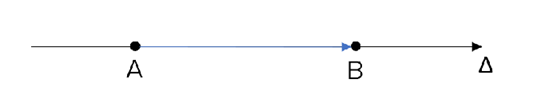
\includegraphics{img/axisdelta_AB.png}
	
	Отрезок оси $\Delta$, ограниченный точками $A$ и $B$, называется \textbf{направленным}, если указано, какая из точек является точкой начала, а какая -- точкой конца отрезка. Если $A$ -- точка начала и $B$ -- точка конца, то направленный отрезок обозначается как $\overline{AB}$.\\
	Направление отрезка также обозначается на рисунке стрелкой.\\\\
	
	Если точки $A$ и $B$ совпадают, то отрезок называется \textit{нулевым} и его направление не определено ($\overline{AA}$).
	\subsection*{Направленные отрезки}
	Два направленных отрезка $\overline{AB}$ и $\overline{CD}$ оси $\Delta$ называется \textbf{равными}, если $A = C$ и $B = D$ ($\overline{AB}$=$\overline{CD}$).\\\\
	Выберем на оси $\Delta$ отрезок в качестве единицы масштаба, тогда можно измерить длину любого отрезка оси $\Delta$.\\
	
	Длина направленного отрезка $\overline{AB}$: |$\overline{AB}$|\\\\
	Если $d(A, B)$ -- расстояние между точками $A$ и $B$, то \[d(A, B) = |\overline{AB}| = |\overline{AB}|\]\\\\
	
	\quad{} Рассмотрим два направленных отрезка $\overline{AB}$ и $\overline{CD}$, которые лежат соответственно на двух параллельных осях $\Delta_1$ и $\Delta_2$. Через точки $A$ и $C$ проведём плоскость $\Pi$, не содержащая точки $B$ и $D$. Эта плоскость $\Pi$ разбивает всё пространство на 2 полупространства.\\
	\quad{} Если точки $B$ и $D$ лежат в одном полупространстве, то говорят, что отрезки $\overline{AB}$ и $\overline{CD}$ \textbf{сонаправленными} и обозначается: $$\overline{AB} \uparrow\uparrow \overline{CD}$$
	\newtheorem*{Note}{Замечание}
	\begin{Note}
	Если $\overline{AB}$ и $\overline{CD}$ лежат на одной оси $\Delta$, то они сонаправлены, если найдётся такой направленный отрезок $\overline{EF}$, что $\overline{AB} \uparrow\uparrow \overline{EF}$ и $\overline{CD} \uparrow\uparrow \overline{EF}$.
	\end{Note}
	Отрезки $\overline{AB}$ и $\overline{CD}$ называются \textit{противоположно направленными} ($\overline{AB} \uparrow\downarrow \overline{CD}$), если $$\overline{AB} \uparrow\uparrow \overline{DC}$$
	\newtheorem*{Def1}{Определение}
	\begin{Def1}
		\underline{Величиной} направленного отрезка $\overline{AB}$ называется неотрицательное действительное число $AB$ и определяется по формуле:
	\end{Def1}
	\begin{equation}\label{1.1}
		AB ::= \left\{
		\begin{split}
			|\overline{AB}|, \overline{AB} \uparrow\uparrow \Delta \\
			-|\overline{AB}|, \overline{AB} \uparrow\downarrow \Delta
		\end{split}\right. \tag{1}
	\end{equation}
	\newtheorem*{Th1}{Теорема 1}
	\begin{Th1}[Шаля]\label{thShal}
		Для любых трёх точек $A$, $B$, $C$ оси $\Delta$ верно равенство
		\begin{equation}\label{1.2}
			AB + BC = AC \tag{2}
		\end{equation}
	\end{Th1}
	\begin{flushleft}
		$\blacklozenge$ \quad{}
		Для взаимного расположения точек $A$, $B$, $C$ возможны 6 ситуаций:
	\end{flushleft}
	\begin{enumerate}
		\item $\overline{AB} \uparrow\uparrow \Delta$, $\overline{BC} \uparrow\uparrow \Delta$\\
		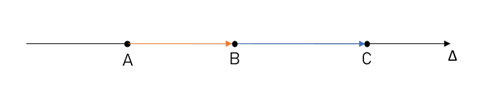
\includegraphics{img/conapr1.png}\\
		$AB+BC$ = [$AB = |\overline{AB}|$, $BC = |\overline{BC}|$] = $|\overline{AB}|+|\overline{BC}|$ = $|\overline{AC}|$ = $AC$\\
		
		\item $\overline{AB} \uparrow\uparrow \overline{BC} \uparrow\downarrow \Delta$\\
		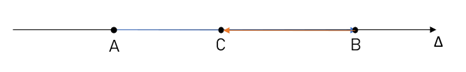
\includegraphics{img/conapr2.png}\\
		$AB+BC$ = [$AB = -|\overline{AB}|$, $BC = -|\overline{BC}|$] = $-|\overline{AB}|-|\overline{BC}|$ = $-(|\overline{AB}|+|\overline{BC}|)$ = $-|\overline{AC}|$ = $AC$\\
		
		\item $\overline{AB} \uparrow\uparrow \Delta, \overline{BC} \uparrow\downarrow \Delta, AB > BC$\\
		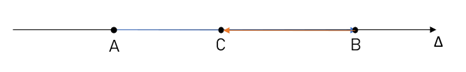
\includegraphics{img/conapr3.png}\\
		$AB+BC$ = [$AB = |\overline{AB}|$, $BC = -|\overline{BC}|$] = $|\overline{AB}|-|\overline{BC}|$ = $|\overline{AC}|$ = $AC$\\
		
		\item $\overline{AB} \uparrow\uparrow \Delta, \overline{BC} \uparrow\downarrow \Delta, AB < BC$\\
		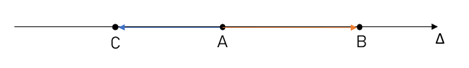
\includegraphics{img/conapr4.png}\\
		$AB+BC$ = [$AB = |\overline{AB}|$, $BC = -|\overline{BC}|$] = $|\overline{AB}|-|\overline{BC}|$ = $-|\overline{AC}|$ = $AC$\\
		
		\item $\overline{AB} \uparrow\downarrow \Delta, \overline{BC} \uparrow\uparrow \Delta, AB > BC$\\
		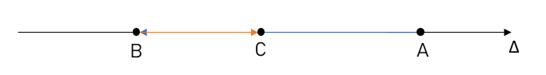
\includegraphics{img/conapr5.png}\\
		$AB+BC$ = [$AB = -|\overline{AB}|$, $BC = |\overline{BC}|$] = $-|\overline{AB}|+|\overline{BC}|$ = $-|\overline{AC}|$ = $AC$\\
		
		\item $\overline{AB} \uparrow\downarrow \Delta, \overline{BC} \uparrow\uparrow \Delta, AB < BC$\\
		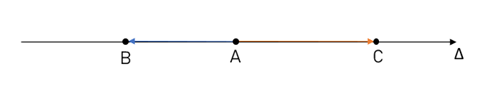
\includegraphics{img/conapr6.png}\\
		$AB+BC$ = [$AB = -|\overline{AB}|$, $BC = |\overline{BC}|$] = $-|\overline{AB}|+|\overline{BC}|$ = $|\overline{AC}|$ = $AC$\\
	\end{enumerate}
	$\hfill\blacksquare$
	
	\quad{} Введём декартову систему координат. На оси $\Delta$ зададим точку $O$, которую назовём \textit{началом отсчёта}, или \textbf{началом координат}. Возьмём [$O$, $E$]  в качестве единицы масштаба.\\
	
	\quad{} Ось, на которой заданы точка начала отсчёта и единица масштаба, называется \textit{координатной осью}. Полупрямая, исходящая из точки $O$ в положительном направлении, называется \textit{положительной полуосью}, а исходящая в отрицательном направлении - \textit{отрицательной полуосью}.
	
	Рассмотрим на координатной оси $\Delta$ точку $A$.
	\newtheorem*{Def2}{Определение}
	\begin{Def2}
		\underline{Координата} $x_A$ точки $A$ ($A(x_A)$) --- величина $OA$ направленного отрезка $\overline{AB}$, т. е. 
		\begin{equation}\label{1.3}
			x_A ::= OA \tag{3}
		\end{equation}
	\end{Def2}
	\quad{} $f: \Delta \longrightarrow \mathbb{R}$ --- отображение\footnote{Это отображение является \textit{взаимно-однозначным}} точек оси $\Delta$ в множество действительных чисел $\mathbb{R}$\\
	\newtheorem*{Th2}{Теорема 2}
	\begin{Th2}
		Для любых точек $A$ и $B$ координатной оси $\Delta$ верно:
		\begin{equation}\label{1.4}
			AB = x_B - x_A \tag{4}
		\end{equation}
		\begin{equation}\label{1.5}
			|\overline{AB}| = |x_B - x_A| \tag{5}
		\end{equation}
	\end{Th2}
	$\blacklozenge$ \quad{} На основании \textbf{Теоремы Шаля}\\
	$$OA + AB = OB \Rightarrow AB = OB - OA \Rightarrow AB = x_B - x_A$$
	(\ref{1.5}) следует из (\ref{1.4}) и того, что длина $|\overline{AB}|$ -- это модуль величины этого отрезка.
	$\hfill\blacksquare$
	
	\subsection*{Деление отрезков в заданном отношении}
	\quad{} Рассмотрим на координатной оси $\Delta$ три точки $A$, $B$, $C$ ($A \ne B$) и \textit{некоторое число} $\lambda \in \mathbb{R}$. Точка $C$ делит направленный отрезок $\overline{AB}$ в отношении $\lambda$, если выполняется: 
	\begin{equation}\label{1.6}
		AC = \lambda CB \tag{6}
	\end{equation}
	
	\subsection*{Замечания.}
	\begin{enumerate}
		\item $C \ne B$\\\\
		Если $C = B$, то из (\ref{1.6}) следует, что $$AB = \lambda BB \Rightarrow AB = 0 \Rightarrow A = B$$ \textbf{Противоречие!}
			
		\item 
		Если $C = A$, то из (\ref{1.6}) следует, что $$AA = \lambda AB \Rightarrow \lambda AB = 0 \Rightarrow \lambda = 0$$
			
		\item $\lambda \ne -1$\\\\
		Если $\lambda = -1$, то из (\ref{1.6}) следует, что $$AC = -CB (BC) \Rightarrow A = B$$ \textbf{Противоречие!}
		
		\item Если $\lambda > 0$, то точка C делит отрезок $\overline{AB}$ \textit{внутренним образом}.\\
		Если $\lambda < 0$, то точка C делит отрезок $\overline{AB}$ \textit{внешним образом}.\\
	\end{enumerate}
	\quad{} Найдем координаты $x_C$ точки $C$, если известны координаты $x_A$ и $x_B$.\\\\
	Рассмотрим равенство (\ref{1.6}): $x_C - x_A = \lambda (x_B - x_C) \Leftrightarrow x_C + \lambda x_C = x_A + x_B \Leftrightarrow$ 
	\begin{equation}\label{1.7}
		\boxed{x_C = \frac{x_A + \lambda  x_B}{1 + \lambda}} \tag{7}
	\end{equation}
	\begin{equation}\label{1.8}
		\lambda = 1 \Rightarrow x_C = \frac{x_A + x_B}{2} \tag{8}
	\end{equation}
	
	\section{Система координат на плоскости}
	\subsection{Декартова прямоугольная система координат (ДПСК)}
	\quad{} Если на плоскости $\Pi$ зафиксировать \textit{две взаимно-перпендикулярные координатные оси} с серединой $O$ - \textit{точкой начала отсчёта}, то говорят, что на плоскости $\Pi$ задана прямоугольная система координат.\\\\
	\begin{center}
		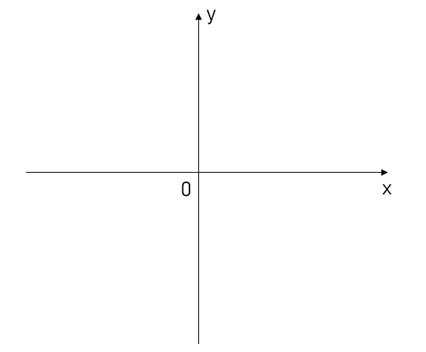
\includegraphics{img/Oxy.png}\\
	    $O_x$ -- ось абсцисс 
		\quad{} $O_y$ -- ось ординат \\ 
		\quad{} \textbf{ДПСК $O_{xy}$}
	\end{center}
	\quad{} Рассмотрим на плоскости $\Pi$ некоторую точку $A$. Ортогональным образом спроецируем её на координатные оси $O_x$ и $O_y$ и получим соответственно точки $A_x$ и $A_y$.\\\\
	\textit{Декартовыми прямоугольными координатами} точки $A$ называются величины направленных отрезков $\overline{OA_x}$ и $\overline{OA_y}$, т. е.
		$$x_A ::= OA_x$$
		$$y_A ::= OA_y$$
	\quad{} Запись $A(x_A, y_A)$ означает, что $(x_A, y_A)$ -- величины декартовых прямоугольных координат точки $A$.\\\\
	\quad{} Таким образом, каждой точке на плоскости $\Pi$ ставится упорядоченная пара из двух декартовых координат этой точки.\\
	Верно и обратное: $$f: \Pi \longrightarrow \mathbb{R}$$\\
	\begin{center}
		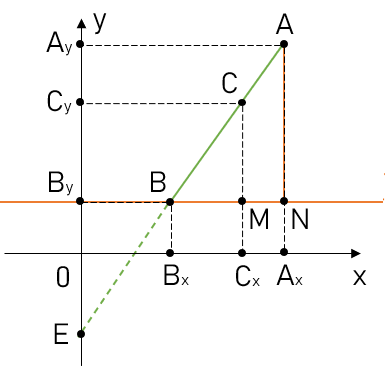
\includegraphics{img/1.2.1 C between AB.png}\\
	\end{center}
	Расмотрим на плоскости $\Pi$ ещё точку $B (x_B, y_B)$. Найти $d(A, B) = |\overline{AB}|$ \\\\	
	$\blacktriangleright$ Ортогональным образом спроецируем точки $A$ и $B$ на координатные оси $O_x$ и $O_y$. Получим точки $A_x, A_y, B_x, B_y$.
	$$|\overline{AN}| = |\overline{A_xB_x}| = |x_B - x_A|$$
	$$|\overline{BN}| = |\overline{A_yB_y}| = |y_B - y_A|$$
	Тогда по теореме Пифагора для $\bigtriangleup$$ANB$ получаем:
	\begin{equation}\label{1.9}
		d(A, B) = |\overline{AB}| = \sqrt{(x_B - x_A)^2 + (y_B - y_A)^2} \tag{9}
	\end{equation}
	\newtheorem*{Th3}{Теорема 3}
	\begin{Th3}
		Координаты $(x_C, y_C)$ точки $C$, делящей направленный отрезок $\overline{AB} (B \ne C)$ в отношении $\lambda = \frac{AC}{BC}$, равны:
		\begin{equation}\label{1.10}
			\left.
			\boxed{\begin{aligned}
				x_C = \frac{x_A + \lambda x_B}{1 + \lambda} \\
				y_C = \frac{y_A + \lambda y_B}{1 + \lambda}
			\end{aligned}}
			\right. \tag{10}
		\end{equation}
	\end{Th3}
	$\blacklozenge$ \quad{} Проектируем точки $A, B, C$ на $O_x, O_y$ и воспользуемся \textit{Теоремой Фалеса} (см. чертёж)\\\\
	\qquad{} Рассмотрим $\bigtriangleup$$ABN$:
	$$AN || CM \Rightarrow \frac{AC}{CB} = \frac{NM}{MB} = \lambda$$
	$$\frac{NM}{MB} = \frac{A_xC_x}{C_xB_x} = \frac{x_A - x_C}{x_C - x_B} = \lambda \Leftrightarrow x_A - x_C = \lambda x_C - \lambda x_B \Leftrightarrow x_C (1 + \lambda) = x_A + \lambda x_B \Leftrightarrow x_C = \frac{x_A + \lambda x_B}{1 + \lambda}$$ \\
	Аналогично для $\bigtriangleup$$AA_yE$: 
	$$AA_y || BB_y || CC_y \Leftrightarrow \frac{y_A - y_C}{y_C - y_B} = \lambda \Leftrightarrow y_C = \frac{y_A + \lambda y_B}{1 + \lambda}$$ $\hfill\blacksquare$
	
	\subsection{Полярная система координат}
	\quad{} Зафиксируем на плоскости $\Pi$ некоторую точку $O$, которую назовём \textit{полюсом}, и луч $OM$, который назовём \textit{полярной осью}. На ней выберем некоторый отрезок в качестве единицы масштаба.\\
	
	Рассмотрим некоторую точку $A$ на плоскости $Pi$ и проведём луч $OA$. 
	\begin{center}
		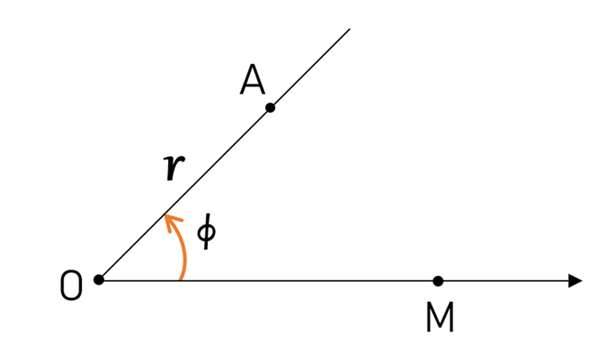
\includegraphics{img/1.2.2 polar axis.png}
	\end{center}
	Тогда точке $A$ можно поставить в соответствие пару чисел $(r, \varphi)$ - ее \textbf{полярные координаты}, где
	\begin{center}
		$r = d(O, A), \underline{0 \le r < +\infty}$\\
		$\varphi$ - угол, на который нужно повернуть полярную ось, чтобы она совпала с лучом $OA$
		(поворот провтив часовой стрелки - \textit{положительное} направление, по часовой стрелке - \textit{отрицательное}), $\underline{\varphi \in \mathbb{R}}$
	\end{center}
	
	Ясно, что если $\varphi$ - полярный угол точки $A$, то $\varphi + 2\pi k, k \in \mathbb{Z}$ также является полярным углом точки A. Поэтому значение полярного угла $\underline{-\pi < \varphi \le \pi}$ называется \textbf{главным значением полярного угла} точки $A$.
	
	\subsection{Связь между декартовой и полярной системами координат}
	\quad{} Рассмотрим на плоскости $\Pi$ некоторую прямоугольную декартову систему координат $O_{xy}$ и такую полярную систему координат, что её полюс совпадает с точкой $O$, а полярная ось совпадает с положительной полуосью $O_x$.
	\begin{center}
		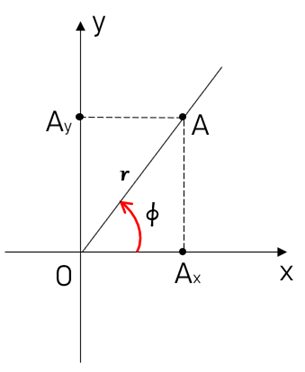
\includegraphics{img/1.2.3 dpsk with polar.png}
	\end{center}
	Нетрудно видеть, что
	\begin{equation}\label{1.11}
		\left\{
		\begin{split}
			x_A = r\cos \varphi \\
			y_A = r\sin \varphi
		\end{split}
		\right. \tag{11}
	\end{equation}
	Из формулы (\ref{1.11}) можно найти \textit{выражения полярных координат точки через её декартовы координаты}, а именно:
	\begin{equation}\label{1.12}
		\boxed{\left\{
		\begin{split}
			r = \sqrt{x_A^2 + y_A^2} \\
			\cos \varphi = \frac{x_A}{\sqrt{x_A^2+y_A^2}} \\
			\sin \varphi = \frac{y_A}{\sqrt{x_A^2+y_A^2}}
		\end{split}
		\right.} \tag{12}
	\end{equation}
	
	\section{Системы координат в пространстве}
	\subsection{Декартова прямоугольная система координат}
	\quad{} Рассмотрим в пространстве \textit{3 взаимно-перпендикулярные ортогональные оси} с единой точкой отсчёта $O$. \\
	Оси образуют 3 координатные плоскости: $O_{xy}, O_{yz}, O_{xz}$. Эти плоскости разбивают пространство на \textit{8 октантов}.
	\begin{center}
		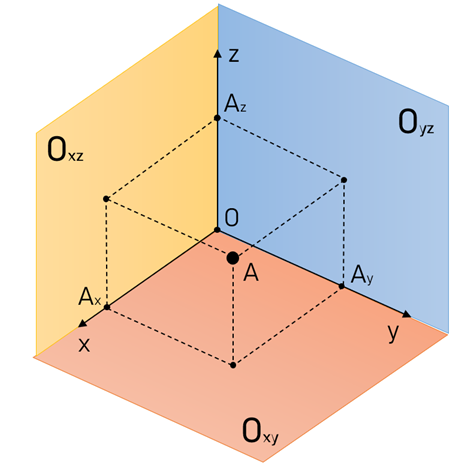
\includegraphics{img/1.3.1 3d dpsk.png}
	\end{center}
	\quad{} Рассмотрим в пространстве точку $A$ и спроецируем ортогональным образом на оси $O_x, O_y, O_z$. Отметим соответствующие точки $A_x, A_y, A_z$.\\\\
	\newtheorem*{Def3}{Определение}
	\begin{Def3}
		\textbf{Декартовыми прямоугольными координатами} точки $A$ в пространстве называются величины отрезков $\overline{OA_x}, \overline{OA_y}, \overline{OA_z}$, т. е.
			$$x_A ::= OA_x$$
			$$y_A ::= OA_y$$
			$$z_A ::= OA_z$$
			$$A (x_A, y_A, z_A)$$
	\end{Def3}
	\newtheorem*{Th4}{Теорема 4}
	\begin{Th4}\label{th4}
		Координаты $(x_C, y_C, z_C)$ точки $C$, делящей отрезок $\overline{AB}$ $(B \ne C)$ в отношении $\lambda = \frac{AC}{CB}$, равны:
		\begin{equation}\label{1.13}
			\left.
			\begin{aligned}
					x_C = \frac{x_A + \lambda x_B}{1 + \lambda} \\
					y_C = \frac{y_A + \lambda y_B}{1 + \lambda} \\
					z_C = \frac{z_A + \lambda z_B}{1 + \lambda}
			\end{aligned}
			\right. \tag{13}
		\end{equation}
	\end{Th4}
	$\blacklozenge$ \quad{}
	Доказательство \textbf{Теоремы 4} аналогично доказательству \textbf{Теоремы 3}
	\begin{equation}\label{1.14}
	d(A, B) = |\overline{AB}| = \sqrt{(x_B - x_A)^2 + (y_B - y_A)^2 + (z_B - z_A)^2} \tag{14}
	\end{equation}
	$\hfill\blacksquare$
	
\end{document}